\documentclass[titlepage]{article}

\usepackage{graphicx} % For images
\usepackage{float}    % For tables and other floats
\usepackage{verbatim} % For comments and other
\usepackage{amsmath}  % For math
\usepackage{amssymb}  % For more math
\usepackage{fullpage} % Set margins and place page numbers at bottom center
\usepackage{listings} % For source code
\usepackage{subfig}   % For subfigures
\usepackage[usenames,dvipsnames]{color} % For colors and names
\usepackage[hidelinks]{hyperref}           % For hyperlinks and indexing the PDF
\usepackage{libertine}
\usepackage{fontenc}
\usepackage[scaled]{beramono}
%\usepackage{lmodern}
%\usepackage{tgadventor}
\usepackage{multicol}

\hypersetup{ % play with the different link colors here
     %colorlinks = true,
     linkcolor = blue,
     frenchlinks = true
      }
      

\begin{document}


% title page/cover
\begin{titlepage}
\begin{center}

{\Huge 
Uplink User-Assisted Relaying \\ in Cellular Networks 
}~\\[4cm]

% The '~' is needed because \\ only works if a paragraph has started.

{\large 
Dual Degree Project 1st Stage Report
}~\\[2cm]

\end{center}

\begin{multicols}{2}
\begin{flushleft}
{\large
\textit{Student:} \\
\text{Prudhvi Porandla} \\
\text{110070039}
}
\end{flushleft}
\columnbreak
\begin{flushright}
{\large
\textit{Guide:} \\
\text{Prof. S. N. Merchant}
}
\end{flushright}
\end{multicols}

\vfill

\begin{center}

\includegraphics[width=4cm]{figures/iitbblack.jpg}~\\[1cm]

{\large
Department of Electrical Engineering\\
Indian Institute of Technology Bombay\\
Mumbai - 400076\\
}

\end{center}
\end{titlepage}
% cover page end
\pagenumbering{roman}


\begin{abstract}
Currently, there are 31,254 level crossings and around 40\% of them are unmanned. The unmanned
crossings are responsible for the maximum number of train accidents. The m
ain objective of this project
is to reduce the number of such accidents by building a reliable system th
at can consistently detect a train
moving towards the crossing and sets off an alarm at the crossing.
\end{abstract}


\tableofcontents
\newpage
%\mbox{}
%\newpage





\section{Introduction}
The solution to this problem is to build a system that can turn on an alarm at the crossing at least 1 min
before the train reaches the crossing and turn off the alarm when the train passes the crossing. To do this, we
designed a sensor unit, using two inductive proximity sensors, that can detect a train and its direction,
and an alarm unit. The sensor unit will be placed 1.5 km away from the crossing while the alarm unit will be
placed at the crossing. When a train passes over the two sensors of the sensor unit, it detects the direction
of the train, counts the number of axles\footnotemark\footnotetext{We actually count the number of wheels on one side, 4 wheels on each side $\implies$ 4 axles}($n$) and sends this information to the alarm unit. If the train is moving
towards the crossing, alarm unit turns on the alarm. When the train passes over the single sensor placed at the crossing,
the alarm unit down counts the number of axles from $n$ and turns off the alarm when the count reaches 0.
\\ \\
In the next sections we present the block and circuit diagrams of various units of the system, different
algorithms used to detect the direction of train and also how false alarm cases are handled.
\subsection{Motivation}
\subsection{Work Reported}
\subsection{Organization of this report}
\pagenumbering{arabic}

\section{Partial Decode-and-Forward Relaying}
\subsection{Functional Block Diagram}


\subsection{Communication unit}
Functions:
\begin{enumerate}
  \item Check if communication link is active
  \item Data transfer
\end{enumerate}

\subsubsection{Link check}
We are using a watchdog timer at the alarm unit to check if the communication
link
between sensor unit and alarm unit is active.

\begin{itemize}
\item Sensor unit triggers by sending some packet (char `A') to alarm unit,
when alarm unit
receives this packet it initializes timer (t=0), when timer = T (t=T) it
resets \texttt{Linkflag}
(\texttt{Linkflag}=0).
\item Sensor unit will trigger every t1 sec and alarm unit initializes timer
to zero (t=0) setting
the \texttt{Linkflag} high (\texttt{Linkflag}=1). In this process \texttt{
Linkflag} stays high (\texttt{Linkflag}=1) as long
as the communication link is active.
\item \texttt{Linkflag} is low (\texttt{Linkflag}=0) implies that it did not
receive any packet for the last T sec and the link in not active.
\end{itemize}
\subsubsection{Data Transfer}
In our application only sensor unit transmits and alarm unit receives. Sensor
unit transmits the
following signals.
\begin{itemize}
\item Alarm on signal `D' when train is detected
\item Axle count `W'
\item Sensor unit active signal `A'
\item False alarm signal `F' in case of false alarm
\end{itemize}

\begin{figure}[H]
\begin{center}
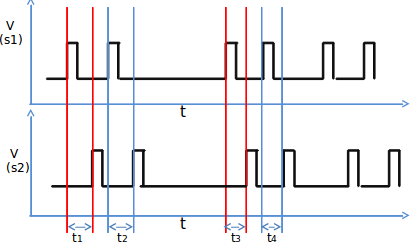
\includegraphics[height = 2in,width=4in,angle=00]{figures/8w_no_miss.png}
\caption{\small pulses on s1, s2 as train crosses the sensor unit}
\end{center}
\end{figure}


\section{Simulations and Results}

\section{Conclusions and Future Work}

\section{References}

\end{document}
